\documentclass[a4paper,10pt]{article}
\usepackage{amsmath}
\usepackage{array}
\usepackage{graphicx}
\usepackage{longtable}
\usepackage{tabularx}
\usepackage{url}
\usepackage[hidelinks]{hyperref}
\renewcommand{\UrlBreaks}{\do\/\do\_\do\.}

% The node's TeX installation has no geometry/booktabs/caption packages.
\setlength{\textwidth}{6.4in}
\setlength{\oddsidemargin}{-0.07in}
\setlength{\evensidemargin}{-0.07in}
\setlength{\topmargin}{-0.55in}
\setlength{\textheight}{9.6in}
\setlength{\parindent}{0pt}
\setlength{\parskip}{0.5em}
\renewcommand{\arraystretch}{1.12}
\graphicspath{{figures/}}

\newcommand{\garnet}{\texttt{GARNET}}
\newcommand{\code}[1]{\texttt{#1}}
\newcommand{\tablefile}[1]{\begin{center}\resizebox{\ifdim\width>\textwidth\textwidth\else\width\fi}{!}{\input{tables/#1}}\end{center}}

\title{\textbf{SP$_N$ and SDP$_N$ Verification and Validation}\\
\large Brantley--Larsen and C5G7 against Carre\~no et al.\ (2024)}
\author{\garnet{} V\&V report, audit item O10}
\date{30 October 2026}

\begin{document}
\maketitle

\section*{Summary}

This report verifies \garnet's SP$_N$ and SDP$_N$ solvers against the two
two-dimensional problems of Carre\~no et al.\ (2024), the paper whose
equations they implement, after the October 2026 code audit (item O10).

\begin{itemize}
\item \textbf{Brantley--Larsen, code verification.} With the paper's coupled
  Marshak vacuum, \garnet's mesh limits equal the paper's Table~6 within
  0.6~pcm for SP1, SP3, SP5, SP7, SDP1 and SDP2. Convergence is second order
  (observed 1.93--2.00), and the extrapolation is good to about 0.2~pcm.
\item \textbf{SDP3 coefficient tables.} The paper's SDP3 results were
  computed with the tables in the authors' FEMFFUSION code: with them,
  \garnet{} reproduces Table~6 within 0.2~pcm. Those tables differ from the
  paper's printed Eq.~(A.6) (which gives $+24$~pcm) and from the
  first-principles tables \garnet{} uses ($-10$~pcm on Brantley--Larsen,
  about $-14$~pcm on C5G7).
\item \textbf{C5G7, pin-resolved.} The pin powers reproduce the paper's
  Table~7 AVG and RMSE against the NEA MCNP reference within 0.04
  percentage points (AVG 1.43\% for diffusion down to 0.53--0.57\% for SP5,
  SP7 and SDP2). The eigenvalues are 11--22~pcm below the paper's (42~pcm
  for SDP3 with \garnet's tables), a model difference of 3--5\% of the
  angular error whose source is not identified. Both codes
  show the paper's C5G7 conclusion: $k$ stagnates with angular order while
  the pin powers improve.
\item \textbf{Flux shapes.} Along the lines the paper plots, \garnet{} agrees
  with the OpenMOC and OpenMC profiles as closely as the paper's own
  solutions do (0.4\% of the peak on Brantley--Larsen, 1.1--1.7\% on C5G7
  for SDP3).
\item \textbf{Findings for the code} (Section~\ref{sec:findings}): the
  per-moment Robin vacuum, then the default of every solver except SP3, is
  52--73~pcm low on a leaky core, so Marshak is now the default wherever it is
  available, with Robin kept for comparison; the C5G7 builder's sampled pin
  areas misstate the fuel inventory and move $k$ by up to 226~pcm (exact areas
  are now an option); and the non-symmetric SDP$_N$ solve failed to converge
  at 2.7 million cells.
\item \textbf{Tests.} The Brantley--Larsen mesh-limit test now covers every
  method at 4~pcm (was SP3 and SDP1 at 10~pcm); a slow pin-resolved C5G7
  test checks diffusion against the paper's $k$ and pin powers.
\end{itemize}


\section{Scope and references}

The reference is A.~Carre\~no, A.~Vidal-Ferr\`andiz, D.~Ginestar and G.~Verd\'u,
``Development of a diffusive simplified double P$_N$ approximation to the
neutron transport equation'', \emph{Ann.\ Nucl.\ Energy} 207 (2024) 110675
(CC BY 4.0, in \code{literature/}). \garnet's SP$_N$ ($N = 1, 3, 5, 7$) and
SDP$_N$ ($N = 1, 2, 3$) solvers implement the same equations in the same
unified form. The paper solves them with second-degree finite elements;
\garnet{} uses cell-centred finite volumes. Two of the paper's problems are
used:

\begin{itemize}
\item \textbf{Brantley--Larsen} (paper Sec.~4.2): one group, three fuel bars
  in a $10 \times 10$~cm moderator square, reflective at $x = 0$ and $y = 0$,
  vacuum at $x = 10$ and $y = 10$ (paper Fig.~3, Table~5). References: the
  paper's own SP$_N$/SDP$_N$ eigenvalues (Table~6), OpenMOC
  ($k = 0.80536$) and TWODANT S$_{16}$ ($k = 0.80613$), and the OpenMOC flux
  along $y = 4.5$~cm (Fig.~4).
\item \textbf{C5G7} (paper Sec.~4.3): the OECD/NEA two-dimensional
  quarter core, seven groups, vacuum outer boundary (Fig.~5). References: the
  paper's eigenvalues and pin-power errors (Table~7), MCNP
  ($k = 1.18655$), the NEA MCNP pin powers, and the OpenMC flux along two
  assembly diagonals (Figs.~6--7).
\end{itemize}

Three questions are separated. \emph{Solution verification}: how far each
\garnet{} eigenvalue is from its own mesh limit. \emph{Code verification}:
whether the mesh-converged \garnet{} result equals the paper's solution of
the same equations. \emph{Validation of the approximation}: how far SP$_N$
and SDP$_N$ are from transport. The last is a property of the equations, so
\garnet{} should reproduce the paper's distance from transport rather than
improve on it.

\section{Code, models and metrics}

\textbf{Code state.} Commit \code{20967d3} (the merged 2026-10-28 audit)
plus the uncommitted audit work of 29--30 October. The audit changes that
bear on these problems are: the coupled Marshak vacuum is now the default of
the dedicated SP3 solver; plain power iteration stops on an error bound
rather than the last change; non-symmetric SDP$_N$ blocks default to GMRES;
and, added for this study, \code{build\_c5g7\_2d} accepts exact pin areas
(\code{exact\_area=True}) and a vacuum outer boundary
(\code{outer\_bc="vacuum"}). Both new options are off by default, so no
earlier result moves.

\textbf{Discretization.} Cell-centred finite volumes on a uniform Cartesian
mesh, second order where material interfaces lie on cell faces. In the
pin-resolved C5G7 model a cell cut by the $r = 0.54$~cm fuel circle is a
volume blend of pin and water: linear in the reaction cross sections,
harmonic in the diffusion coefficients, and weighted by fission production
in the emission spectrum. Its covered fraction is computed in closed form.
The pin-cell-homogenized model, which \path{tests/validation/test_c5g7.py}
runs, volume-weights each 1.26~cm pin cell instead.

\textbf{Vacuum boundaries.} \emph{Marshak} is the coupled condition
$-\mathbf{n}\cdot D\nabla U = (g \otimes I)\,U$ that the paper uses.
\emph{Robin} applies $\alpha = 1/2$ to each moment separately. SP1 is
diffusion, for which the two coincide. When these runs were made only the
dedicated SP3 solver defaulted to Marshak; following this study (finding~3),
every SP$_N$/SDP$_N$ eigen, transient and noise solver now does so wherever
the coupled term exists, and Robin stays available as
\code{marshak\_vacuum=False}. The dedicated SDP1 solver has no Marshak term
and keeps Robin; its Marshak runs use the general SDP$_N$ block of order~1.
Every run here names its boundary explicitly, so the change of default moves
none of the results.

\textbf{Tolerances.} Brantley--Larsen: \code{tol\_k} $= 10^{-10}$,
\code{tol\_source} $= 10^{-9}$. C5G7: $10^{-9}$ and $10^{-8}$. Every run
converged.

\textbf{Metrics.} Eigenvalue differences are signed,
$10^5 (k - k_{\rm ref})$ in pcm. The paper's Eq.~(49) defines a relative
difference, but its Tables~6 and~7 list $10^5 |k - k_{\rm ref}|$ (for
example SP1 in Table~7: $10^5 \times |1.18336 - 1.18655| = 319$); the
tables are what is compared here. Pin-power errors
$e_i = (P_i - P_i^{\rm ref})/P_i^{\rm ref}$ over the 1056 fuel pins, with
powers normalized to a mean of 1: AVG $= \langle |e_i| \rangle$ (paper
Eq.~50); the paper's RMSE, whose Table~7 values match
$\sqrt{\sum e_i^2}/N$ (Eq.~51 as printed equals AVG); the conventional RMS
$\sqrt{\langle e_i^2 \rangle}$; MRE $= \sum |e_i| P_i^{\rm ref} / \sum
P_i^{\rm ref}$; and the largest $|e_i|$. Flux profiles are compared after a
least-squares scale factor (the paper's flux units are arbitrary), as RMS and
largest deviation in percent of the reference peak.

\textbf{Paper figures.} The paper's plots are vector graphics, so the
reference curves were read from the drawn paths themselves
(\code{extract\_paper\_figures.py}), not digitized from pixels. Axis
calibration is a linear fit through the tick marks; the residual plus half
the line width is below 0.4\% of the curve's peak in all five panels.

\section{Brantley--Larsen}
\label{sec:bl}

\subsection{Problem and runs}

One energy group: fuel $\Sigma_t = 1.5$, $\Sigma_{s0} = 1.35$,
$\nu\Sigma_f = 0.24$~cm$^{-1}$; moderator $\Sigma_t = 1.0$,
$\Sigma_{s0} = 0.93$~cm$^{-1}$ (paper Table~5). The fuel bars occupy
$x \in [1,2] \cup [4,5] \cup [7,8]$, $y \in [0,9]$~cm. Every interface lies on
a cell face for $n$ a multiple of 10, so the finite-volume scheme is second
order. Each method was run with Marshak and Robin vacuum on
$n \times n$ meshes, $n = 40, 80, 160, 320, 640$. The GMRES runs of SDP2
(Marshak) and SDP3 (both boundaries) at $n = 640$ would have taken 8--20~h
each on the shared node and were stopped; for those three the extrapolation
uses $n = 80, 160, 320$.

\subsection{Mesh convergence}

\begin{figure}[h]
\centering
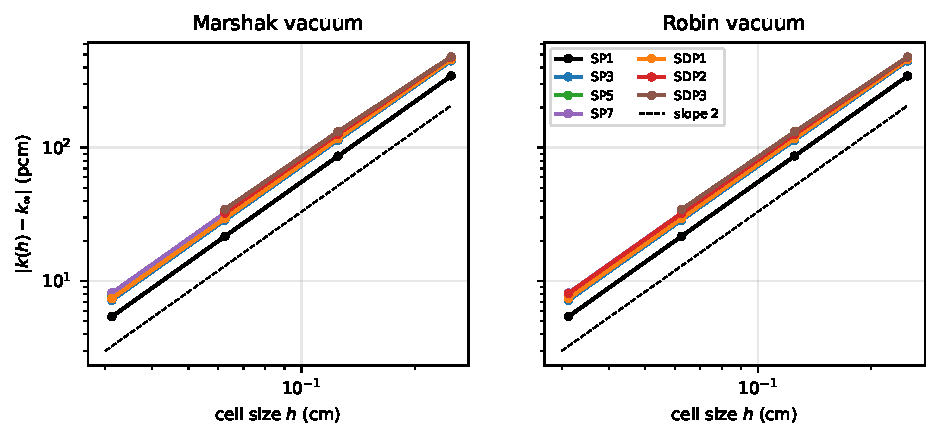
\includegraphics[width=0.82\textwidth]{bl_convergence.pdf}
\caption{Brantley--Larsen: distance of each mesh's $k$ from its own
extrapolated limit. Every method and boundary treatment converges at second
order.}
\label{fig:bl-conv}
\end{figure}

Table~\ref{tab:bl-conv} and Fig.~\ref{fig:bl-conv}. The observed order from
the finest three meshes is between 1.93 and 2.00 for every method and both
vacuum treatments, and $k$ decreases monotonically under refinement.
$k_\infty$ is the Richardson extrapolation with the observed order. The GCI
column is Roache's grid-convergence index with safety factor 1.25; it is
1.7--2.6~pcm where $n = 640$ exists and 10--11~pcm where the triple ends at
$n = 320$. The GCI is a conservative bound: wherever both triples exist
(14 configurations), extrapolating from $n = 80, 160, 320$ and from
$n = 160, 320, 640$ agrees within 0.21~pcm.

\begin{table}[h]
\caption{Brantley--Larsen eigenvalues by mesh, observed order $p$, extrapolated
$k_\infty$ and GCI.}
\label{tab:bl-conv}
\tablefile{bl_convergence}
\end{table}

On the $80 \times 80$ mesh of \path{tests/validation/test_brantley_larsen_2d.py}
the mesh error is $+87$~pcm for SP1 and $+114$ to $+132$~pcm for the
transport methods (Table~\ref{tab:bl-split}). That is larger than the
difference between consecutive SP$_N$ orders above SP5, so single-mesh
comparisons with the paper on that mesh mostly measure mesh error.

\subsection{Comparison with the paper}

\begin{table}[h]
\caption{Brantley--Larsen: extrapolated \garnet{} eigenvalues against the
paper's Table~6 and OpenMOC (pcm). ``Robin $-$ paper'' uses \garnet's
Robin-vacuum $k_\infty$.}
\label{tab:bl-paper}
\tablefile{bl_vs_paper}
\end{table}

\begin{figure}[h]
\centering
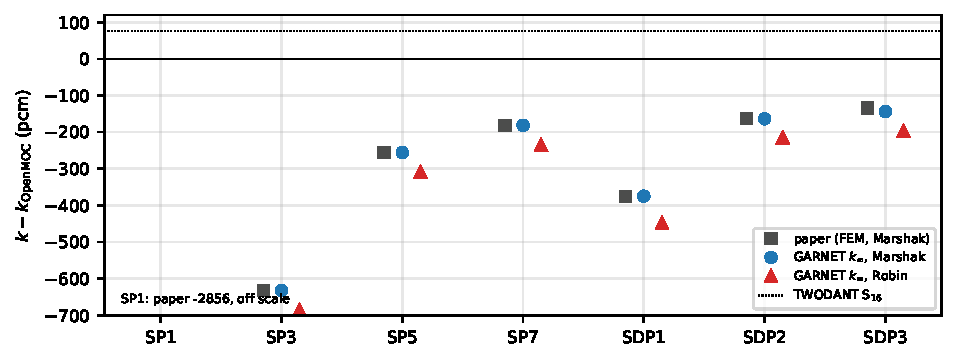
\includegraphics[width=0.82\textwidth]{bl_keff.pdf}
\caption{Brantley--Larsen eigenvalues relative to OpenMOC: paper (finite
elements, Marshak), \garnet{} mesh limit with Marshak and with Robin vacuum.
TWODANT S$_{16}$ is the dotted line.}
\label{fig:bl-k}
\end{figure}

With the Marshak boundary, \garnet's mesh limit equals the paper's Table~6
within 0.6~pcm for SP1, SP3, SP5, SP7, SDP1 and SDP2
(Table~\ref{tab:bl-paper}, Fig.~\ref{fig:bl-k}), about the $\pm 0.5$~pcm
rounding of Table~6. This is the code
verification: the same equations, discretized independently (finite volumes
here, second-degree finite elements in the paper), give the same eigenvalue.

SDP3 is $-9.9$~pcm from the paper. \garnet{} does not use the SDP3
coefficient rows 2--3 printed in the paper's Eq.~(A.6): a from-scratch
symbolic derivation from the paper's own closure reproduces its SDP1 and SDP2
tables and every Marshak matrix exactly, but not those rows
(\path{tests/verification/test_sdpn_derivation.py}, note in
\code{garnet/spn.py}). Section~\ref{sec:a6} shows that the paper's SDP3
values come from a third set, the tables in the authors' FEMFFUSION code,
and that with those \garnet{} reproduces them too.

The Robin vacuum lowers $k$ by 52--54~pcm for every method except SDP1
($-73$~pcm). It was the default of every solver except the dedicated SP3
when this study started; Marshak is now the default wherever it is available,
and Robin is kept for comparison.

The angular error, $k_\infty - k_{\rm OpenMOC}$ with Marshak, is
$-2856$~pcm for diffusion, $-632$, $-256$ and $-181$~pcm for SP3, SP5, SP7,
and $-375$, $-163$ and $-144$~pcm for SDP1, SDP2, SDP3. At equal numbers of
moments SDP$_N$ is closer to transport than SP$_{2N+1}$ (SDP1/SP3,
SDP2/SP5, SDP3/SP7), the paper's central claim, and it holds with the
re-derived SDP3 tables. The two transport references differ by 77~pcm
(TWODANT S$_{16}$ above OpenMOC), which is about half the remaining SDP3 and
SP7 errors: the references do not resolve which of those two is closer to
transport.

\subsection{Error budget on the test mesh}

\begin{table}[h]
\caption{Brantley--Larsen error budget (pcm). Mesh error is $k_{80} - k_\infty$
with Marshak. The last two columns are the single-mesh comparison of the
validation test on the $80 \times 80$ mesh, with each vacuum treatment.}
\label{tab:bl-split}
\tablefile{bl_split}
\end{table}

Table~\ref{tab:bl-split} splits the single-mesh comparison into its parts.
With Marshak, every method is $+87$ to $+127$~pcm above the paper on the
$80 \times 80$ mesh, and all of it is mesh error (for SDP3, less the
$-10$~pcm of its re-derived tables). With Robin the offset is
smaller, $+45$ to $+73$~pcm, only because two errors of opposite sign add:
mesh error and the Robin offset ($-52$ to $-73$~pcm). Under the old Robin
defaults the test's 150~pcm envelope therefore passed partly by
cancellation; it now checks the Marshak results, and the Robin offset
separately.

\subsection{Equivalent code paths}

\begin{table}[h]
\caption{Dedicated solvers against the general SP$_N$/SDP$_N$ block of the same order.}
\label{tab:bl-eq}
\tablefile{bl_equivalence}
\end{table}

SP3 and SDP1 each have a dedicated two-moment solver and can also be run
through the general block of order 1 (Table~\ref{tab:bl-eq}). With Marshak,
the dedicated SP3 solver and the SP$_N$ block agree to $2 \times 10^{-10}$ on
every mesh: two independent implementations of the coupled boundary. With
Robin they differ by up to 0.7~pcm (SP3) and 0.35~pcm (SDP1), because the
dedicated solvers apply $\alpha = 1/2$ to $(\Phi_1, \phi_2)$ and the general
block to its $U$ moments. The per-moment Robin term is an approximation
whose result depends on the choice of moments; the Marshak condition is not.

\subsection{Flux along $y = 4.5$~cm}

\begin{figure}[h]
\centering
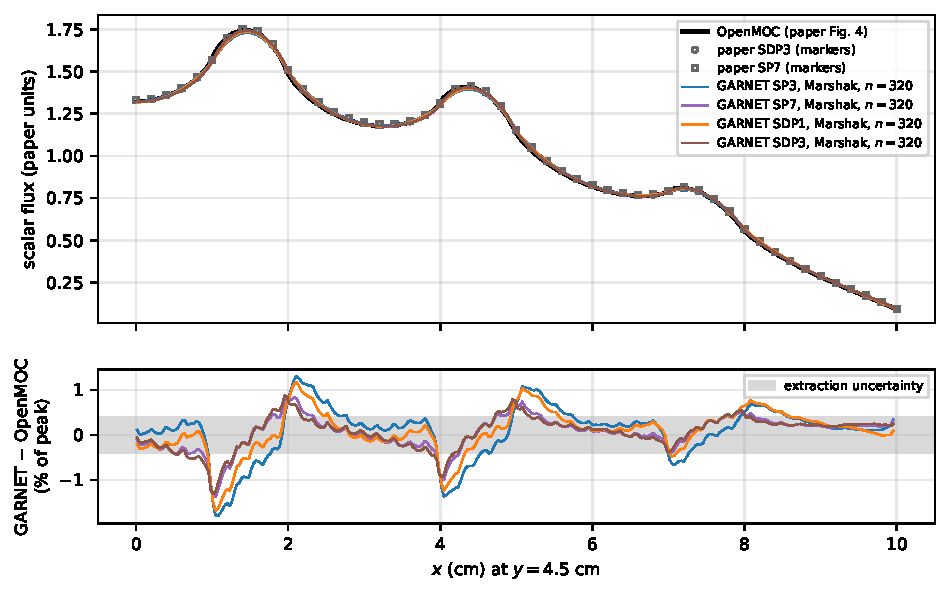
\includegraphics[width=0.85\textwidth]{bl_flux_line.pdf}
\caption{Scalar flux along $y = 4.5$~cm: OpenMOC and the paper's SDP3 and SP7
markers (paper Fig.~4) and \garnet{} with Marshak vacuum. \garnet{} curves are
scaled to OpenMOC by least squares. Lower panel: \garnet{} minus OpenMOC; the
grey band is the extraction uncertainty.}
\label{fig:bl-flux}
\end{figure}

\begin{table}[h]
\caption{Flux along $y = 4.5$~cm against OpenMOC, after a least-squares scale
(\% of the OpenMOC peak).}
\label{tab:bl-flux}
\tablefile{bl_flux}
\end{table}

Fig.~\ref{fig:bl-flux} and Table~\ref{tab:bl-flux}. \garnet's SDP3 and SP7
deviate from OpenMOC by 0.36--0.37\% of the peak (RMS), the paper's own SDP3
and SP7 markers by 0.39--0.40\%. Both are at the extraction uncertainty
(0.39\%), so on this line the two codes agree with transport equally well.
The remaining structure, up to 1.8\% of the peak, sits at the fuel-bar edges,
where the angular flux is most anisotropic; SP3 is the largest there and SDP3
the smallest. The paper's markers, 0.2~cm apart, are too sparse to show it.

\subsection{The paper's printed SDP3 tables}
\label{sec:a6}

Three sets of SDP3 coefficient tables are in circulation, and they differ only
in the closure rows 2--3:

\begin{itemize}
\item \textbf{Re-derived} (\garnet's default): rows 2--3 obtained symbolically
  from the paper's own closure, Eq.~(34). The same derivation reproduces the
  paper's SDP1 and SDP2 tables and all three Marshak matrices exactly.
\item \textbf{FEMFFUSION}: the tables in the authors' code
  (\path{src/matrix_operators/matrix_operators_sdpn.cc}).
\item \textbf{Paper (A.6)}: the tables as printed. They equal FEMFFUSION's
  except row 2 of $c^{(3)}$, printed as $(36/55,\ 54/175)$ where the code has
  $(9/25,\ -54/175)$.
\end{itemize}

\begin{table}[h]
\caption{Brantley--Larsen SDP3 with Marshak vacuum and the three coefficient
sets. $k_\infty$ is extrapolated from $n = 80, 160, 320$.}
\label{tab:bl-a6}
\tablefile{bl_sdp3_tables}
\end{table}

On Brantley--Larsen (Table~\ref{tab:bl-a6}) the FEMFFUSION tables give a
mesh limit 0.2~pcm from the paper's 0.80402, the re-derived tables
$-9.9$~pcm and the printed tables $+23.6$~pcm. The paper's SDP3 results were
therefore computed with the FEMFFUSION tables, and with them \garnet{}
reproduces Table~6 for all seven methods. On C5G7 at $s = 4$ the FEMFFUSION
tables raise SDP3 by 14.3~pcm and the printed ones by 15.2~pcm.

Which tables are right is a question of derivation, which this benchmark
cannot settle. The re-derived rows are the only ones of the three that follow
from the closure the paper states, and
\path{tests/verification/test_sdpn_derivation.py} keeps them in place. The
choice moves $k$ by 10--15~pcm on these problems, small against SDP3's
angular error ($-144$~pcm against OpenMOC on Brantley--Larsen).



\subsection{Cost}

\begin{table}[h]
\caption{Brantley--Larsen cost at $n = 160$, best of three solves on one CPU
thread (merlin7 \code{cn000}). Inner iterations are operator applies of the
within-group Krylov solver. The paper's CPU times are for its own $80 \times 80$
finite-element mesh and are listed only for scale.}
\label{tab:bl-cost}
\tablefile{bl_cost}
\end{table}

Table~\ref{tab:bl-cost}. At $n = 160$ (25\,600 cells, one group) the SP$_N$
solves take 0.8--3.8~s with nearly the same inner work for every order
(3088--3357 operator applies): the cost grows with the size of the block,
not with the number of iterations, and the Marshak boundary costs SP$_N$
nothing measurable (CG either way). SDP1 and SDP2 with Robin vacuum are
symmetrized and solved by CG at about the cost of SP3 and SP5. With Marshak
their block is non-symmetric and runs GMRES: 1.5 times the applies but 5--6
times the time (8.0 and 13.0~s), the rest being GMRES's orthogonalization.
SDP3 has no symmetric form once a vacuum face is present and runs GMRES with
either boundary (18--19~s). The paper's CPU times refer to its own mesh and
machine and are listed for scale only.



\section{C5G7}
\label{sec:c5g7}

\subsection{Models and runs}

The quarter core is $51 \times 51$ pin cells of 1.26~cm (four $17 \times 17$
assemblies and a 21.42~cm water reflector), seven groups, reflective on the
two symmetry planes and vacuum outside. Three \garnet{} models were run:

\begin{itemize}
\item \textbf{Pin-resolved} (the paper's geometry): every lattice position is
  an $r = 0.54$~cm cylinder in water, on $s \times s$ cells per pin cell,
  with exact covered fractions (\code{build\_c5g7\_2d(pin\_resolved=True,
  exact\_area=True, outer\_bc="vacuum")}). With Marshak vacuum,
  $s = 4$--$48$ for SP$_N$ and $s = 4$--$24$ for SDP$_N$; Robin vacuum at
  $s = 4, 8, 16$; zero-flux outer faces at $s = 8$.
\item \textbf{Pin-resolved with sampled areas}: the builder's default
  $16 \times 16$-point sampling of the covered fractions, SP1 only.
\item \textbf{Pin-cell homogenized}: each pin cell volume-weighted, zero-flux
  outer faces, $s = 1, 2, 4, 8$. This is the model of
  \path{tests/validation/test_c5g7.py} (at $s = 1$).
\end{itemize}

Up to $s = 12$ runs were made on the CPU, from $s = 8$ on a GH200
(\code{data/runs-gh200/}). The 18 configurations run on both agree to
$1.3 \times 10^{-13}$ in $k$.

\subsection{Mesh convergence}

\begin{figure}[h]
\centering
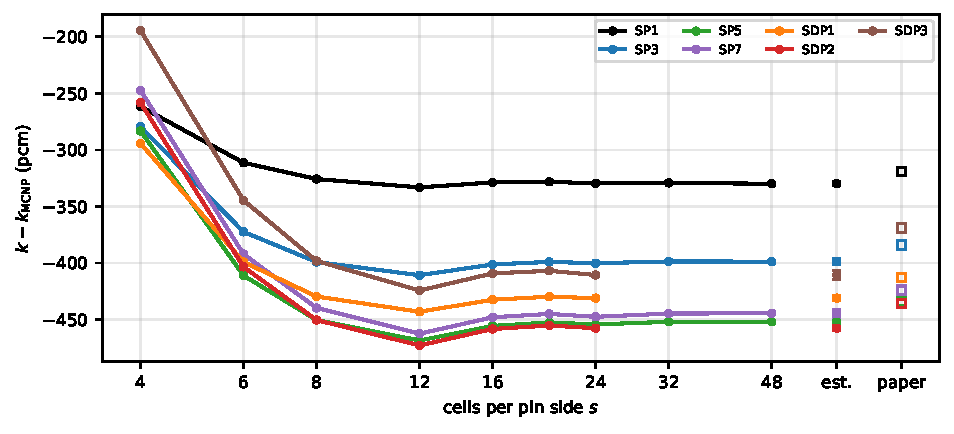
\includegraphics[width=0.85\textwidth]{c5g7_keff.pdf}
\caption{C5G7 pin-resolved, Marshak vacuum: $k - k_{\rm MCNP}$ against cells
per pin side. ``est.'' is the finest-mesh estimate with its spread over
$s \ge 16$; ``paper'' is Table~7.}
\label{fig:c5g7-k}
\end{figure}

The pin-resolved model does not converge monotonically
(Fig.~\ref{fig:c5g7-k}, Table~\ref{tab:c5g7-k}). At $s = 4$ every method is
68--216~pcm above its fine-mesh value; at $s = 12$ every method dips 3--18~pcm
below it; from $s = 16$ on the values settle. How the fuel circle cuts the
cells changes from mesh to mesh, so the blend error does not follow a power
law, and Richardson extrapolation through these points would be arbitrary.
The estimate is therefore the finest-mesh $k$ ($s = 48$ for SP$_N$, 24 for
SDP$_N$). Its uncertainty, 1.7--3.8~pcm, is the larger of two measures: the
largest difference from it among the meshes with $s \ge 16$, and its
distance to a least-squares $k_\infty + b/s^2$ fit over the same meshes.

\begin{table}[h]
\caption{C5G7 pin-resolved eigenvalues, Marshak vacuum. Paper column: Table~7
$k$ and $10^5 (k - k_{\rm MCNP})$. Differences in pcm.}
\label{tab:c5g7-k}
\tablefile{c5g7_keff}
\end{table}

\subsection{Comparison with the paper and MCNP}

For the six methods whose tables the paper and \garnet{} share (SP1--SP7,
SDP1, SDP2), \garnet's estimate is 11--22~pcm below Table~7, and the offset
grows with the number of moments: 11~pcm for diffusion, 15--20~pcm for
SP3--SP7, 18--22~pcm for SDP1--SDP2. For SDP3 it is 42~pcm. The FEMFFUSION
tables raise C5G7 SDP3 by 14~pcm at $s = 4$ (Section~\ref{sec:a6}), so with
them the offset would be about 27~pcm, in line with the other methods.

Unlike Brantley--Larsen, the two C5G7 models are not the same discrete
problem. The paper meshes each pin with second-degree finite elements
(its Fig.~5) and states neither how the circular pin boundary is represented
nor a mesh study; \garnet{} blends the cells the circle cuts, with exact
areas. The source of the 11--22~pcm offset is not identified. It is 3--5\% of
the 320--460~pcm angular error and changes none of the orderings below.

Against MCNP both codes give the same picture. Diffusion is closest
($-330$~pcm here, $-319$~pcm in the paper), and every SP$_N$ and SDP$_N$
order is further away ($-399$ to $-458$~pcm here, $-369$ to $-436$~pcm in the
paper). This is the stagnation the paper reports for C5G7: on this
lightly heterogeneous lattice, the eigenvalue is not a measure of angular
accuracy. The pin powers are.


\subsection{Modelling choices}

\begin{table}[h]
\caption{C5G7 at $s = 8$: effect of the vacuum treatment and of pin-cell
homogenization on $k$ (pcm).}
\label{tab:c5g7-eff}
\tablefile{c5g7_effects}
\end{table}

Table~\ref{tab:c5g7-eff}. The vacuum faces sit behind a full assembly width
of water, so the boundary treatment hardly matters here: Robin is 0.2--0.3~pcm
below Marshak, and the builder's default zero-flux faces are 0.2--1.4~pcm
below. The pin-area computation matters much more. With the default sampled
fractions, SP1 is 226~pcm higher at $s = 4$ and 22~pcm lower at $s = 8$ than
with exact fractions, the result of a fuel-area error of $-0.66$\% and
$+0.06$\% (finding~4 explains why sampling errs this way). Pin-cell homogenization raises $k$ by 379~pcm (SP1) to 662~pcm
(SDP2) against the pin-resolved model at the same mesh.

\subsection{Pin powers}

\begin{table}[h]
\caption{C5G7 pin powers against the NEA MCNP reference, Marshak vacuum,
finest mesh. Errors in \%; the paper's Table~7 AVG and RMSE in brackets.
AVG, RMSE as the paper's tables use it ($\sqrt{\sum e_i^2}/N$), RMS, MRE and
the largest pin error, the largest pin power (MCNP 2.498), and the assembly
power errors.}
\label{tab:c5g7-pins}
\tablefile{c5g7_pins}
\end{table}

\begin{figure}[h]
\centering
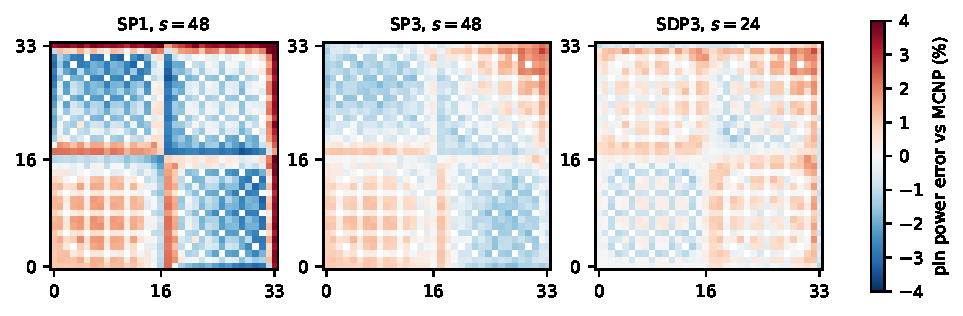
\includegraphics[width=0.85\textwidth]{c5g7_pin_errors.pdf}
\caption{Pin power error against MCNP in the four fuel assemblies (inner
UO$_2$ at the bottom left, MOX on the off-diagonal, outer UO$_2$ at the top
right).}
\label{fig:c5g7-pins}
\end{figure}

Table~\ref{tab:c5g7-pins} and Fig.~\ref{fig:c5g7-pins}. Unlike $k$, the pin
powers improve with angular order: AVG falls from 1.43\% for diffusion to
0.74\% for SP3, 0.66\% for SDP1 and 0.53--0.57\% for SP5, SP7, SDP2 and
SDP3. These are the paper's Table~7 values within 0.04 percentage points
for SP1 to SP7, SDP1 and SDP2 (SP1 1.43 against 1.43, SP3 0.74
against 0.75), and the paper's RMSE measure agrees as well. The agreement
shows that the paper scored its pin powers against the NEA MCNP reference
used here, and that the two codes' solutions match pin by pin, not only in
$k$.

For the higher orders AVG converges with mesh more slowly than $k$ and from
below: SP7 rises from 0.47\% at $s = 8$ to 0.54\% at $s = 48$, SDP3 from
0.49\% at $s = 8$ to 0.56\% at $s = 24$, still climbing. The remaining gap
to the paper for SP7, SDP2 and SDP3 (0.03--0.08 points, largest for SDP3 at
its coarser finest mesh) is consistent with that. Pin-power results from
$s \le 12$ therefore understate the converged error.

The largest pin error is 2.6--2.9\% for every transport method and 5.8\% for
diffusion. In every case it is a corner pin of the outer UO$_2$ assembly next
to the reflector, where the power is lowest (0.23--0.29) and the MCNP
reference itself is least precise. The largest pin power is within 1\% of
MCNP's 2.498, and every assembly power within 0.65\%.


\subsection{Flux along the assembly diagonals}

\begin{figure}[h]
\centering
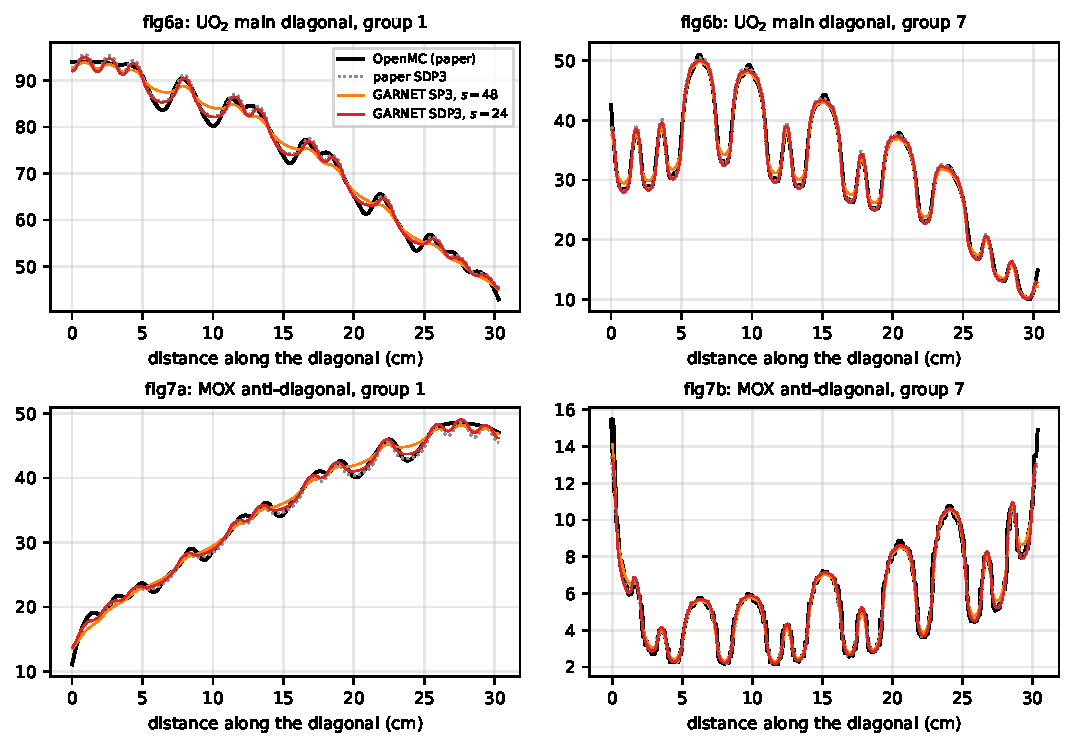
\includegraphics[width=\textwidth]{c5g7_flux_lines.pdf}
\caption{Groups 1 and 7 along the inner UO$_2$ main diagonal (paper Fig.~6)
and the MOX anti-diagonal (Fig.~7): OpenMC and the paper's SDP3, both read
from the paper, and \garnet{} SP3 and SDP3 scaled to OpenMC by least squares.}
\label{fig:c5g7-lines}
\end{figure}

\begin{table}[h]
\caption{Flux along the diagonals against OpenMC, after a least-squares scale
(\% of the OpenMC peak).}
\label{tab:c5g7-lines}
\tablefile{c5g7_flux}
\end{table}

Fig.~\ref{fig:c5g7-lines} and Table~\ref{tab:c5g7-lines}. \garnet's SDP3
deviates from OpenMC by 1.1--1.7\% of the peak (RMS) on the four panels, the
paper's SDP3 by 1.1--2.0\%: the two agree with the Monte Carlo profile equally
well, and \garnet's SDP3 is closer in group~7 of the MOX diagonal (1.7
against 2.0\%). \garnet's SP3 is further away, 1.5--1.9\%, as in the paper's
own SP$_N$/SDP$_N$ comparison. The largest local deviations, up to 8\% of the
peak in group~7, sit on the thermal-flux peaks in the water between pins and
at the reflector-side corner of the MOX assembly. The OpenMC curve is
steepest there, so these are also the points where the extracted reference is
least precise.


\subsection{The homogenized model of the regression test}

\begin{table}[h]
\caption{C5G7 pin-cell homogenized, zero-flux outer faces. $k_\infty$ from
$s = 4, 8$ at second order. Differences in pcm.}
\label{tab:c5g7-hom}
\tablefile{c5g7_homogenized}
\end{table}

The regression test's model, pin-cell homogenized at $s = 1$, lands 8--165~pcm
below MCNP (Table~\ref{tab:c5g7-hom}). The agreement is a cancellation of two
large errors. Homogenizing each pin cell raises $k$ by 380--660~pcm against
the pin-resolved model (Table~\ref{tab:c5g7-eff}), so the homogenized mesh
limit is 57--223~pcm \emph{above} MCNP and 376--650~pcm above the paper; the
$s = 1$ mesh then lowers $k$ by 222--231~pcm. The test's eigenvalue envelopes
(2\% for diffusion, 0.5\% for the family) are therefore not accuracy
statements. What those tests guard is the internal ordering of the hierarchy
and the clustering of the six transport methods, which is where the paper's
SDP2/SDP3 table errors showed.


\subsection{Solver behaviour and cost}

\begin{table}[h]
\caption{C5G7 cost, Marshak vacuum. CPU: best of three at $s = 4$, one
thread. GH200: single runs, which include CuPy kernel compilation on first
use; outer and inner counts at $s = 24$.}
\label{tab:c5g7-cost}
\tablefile{c5g7_cost}
\end{table}

Table~\ref{tab:c5g7-cost}. On one CPU thread at $s = 4$ (41\,616 cells,
seven groups) the SP$_N$ solves take 6--40~s and the SDP$_N$ solves
49--124~s. With Marshak vacuum every SDP$_N$ block is non-symmetric and runs
GMRES. At $s = 4$ its outer iteration count is still close to SP$_N$'s (64--106
against 59--68), but from $s = 8$ on it roughly doubles (121--161 against
57--73), and at $s = 24$ the inner applies are 2.9--3.6 times those of
SP3--SP7. On the
GH200 at $s = 24$ (1.5 million cells) SP$_N$ takes 30--271~s and SDP$_N$
1580--1969~s. At $s = 32$ none of the SDP$_N$ solves converged: in the first
outer iteration GMRES with Jacobi preconditioning stopped at 5000 iterations,
1.3--4.8 times above its tolerance (finding~5 in
Section~\ref{sec:findings}). The SP$_N$ solves ran to $s = 48$ (6.0 million
cells) in 2--14 minutes each.

The pin-resolved study is a GPU calculation: on the shared CPU node, with up
to 16 runs at once, the SP$_N$ solves at $s = 12$ took 14--77 minutes each and
an SDP3 solve at $s = 12$ was projected at over 20 hours.



\clearpage
\section{Test tolerances}
\label{sec:tests}

\textbf{\path{tests/validation/test_brantley_larsen_2d.py}.} The
single-mesh tests now check the Marshak results, the default, on the
$80 \times 80$ mesh: each method within 150~pcm of Table~6 (measured $+87$ to
$+127$~pcm, all mesh error) and a positive offset with a spread below 60~pcm
(measured 41~pcm). A new test keeps the per-moment Robin results for
comparison: Robin minus Marshak between $-80$ and $-45$~pcm (measured $-53$
to $-54$~pcm, and $-73$~pcm for SDP1). Before, the single-mesh tests ran each
solver's default, mostly Robin, and passed partly by cancellation
(Table~\ref{tab:bl-split}). The mesh-limit test was the
weak one: it checked SP3 and SDP1 only, to 10~pcm. It now checks every
method with the Marshak vacuum against Table~6 to 4~pcm, from $n = 80$ and
160 at second order; that two-mesh estimate is within 2.2~pcm of the
three-mesh limits of Table~\ref{tab:bl-conv}, and the measured distances from
the paper are within 1.5~pcm. SP1, SP3, SP5, SP7 and SDP1 run by default
(about 20~s together); SDP2 and SDP3 with the FEMFFUSION tables, which need
GMRES, are marked \code{slow}, as is a test that the re-derived SDP3 stays
4--12~pcm below the paper (measured $-7.9$~pcm from two meshes). A value
near zero there would mean the tables had been changed back to the paper's.

\textbf{\path{tests/validation/test_c5g7.py}.} The homogenized tests keep
their envelopes, with corrected explanations: Section~\ref{sec:c5g7} shows
that their closeness to MCNP is a cancellation, so they guard the ordering
and clustering of the hierarchy, not accuracy. Two tests are new. One checks
that the exact pin areas reproduce $\pi r^2$ at any resolution and that the
builder passes them and the vacuum boundary through. The other, marked
\code{slow} (about a minute), runs pin-resolved diffusion at $s = 8$ with
exact areas and vacuum outside, and checks it against the paper's SP1: $k$
within 10~pcm (measured $-6.8$~pcm) and the pin-power AVG against the NEA
MCNP map within 0.06 percentage points of the paper's 1.43\% (measured
1.46\%). It skips without a FEMFFUSION checkout, which carries that map.


\section{Findings and recommendations}
\label{sec:findings}

\begin{enumerate}
\item \textbf{Code verification passes.} On Brantley--Larsen, with the
  paper's Marshak boundary, \garnet's mesh limits equal Table~6 within
  0.6~pcm for SP1, SP3, SP5, SP7, SDP1 and SDP2, and within 0.2~pcm for SDP3
  run with the authors' FEMFFUSION tables. On C5G7 the pin powers reproduce
  the paper's AVG and RMSE within 0.04 percentage points.

\item \textbf{The paper's SDP3 results use tables that differ from both the
  printed Eq.~(A.6) and the derivation.} The FEMFFUSION tables reproduce the
  paper's SDP3 eigenvalue; the printed ones are 24~pcm off, and \garnet's
  re-derived ones 10~pcm (Brantley--Larsen) to 14~pcm (C5G7) lower.
  \garnet{} keeps the re-derived tables. No code change is needed; the
  difference is documented in \code{garnet/spn.py}.

\item \textbf{The vacuum default was inconsistent across the family;
  Marshak is now the default.} When this study started, only the dedicated
  SP3 solver defaulted to the coupled Marshak condition. SP5, SP7 and the
  SDP$_N$ solvers defaulted to the per-moment Robin term, which is 52--73~pcm
  low on Brantley--Larsen and depends on the moment variables it is applied
  to (0.35--0.7~pcm between equivalent solvers); on a reflected core such as
  C5G7 the choice is irrelevant (0.3~pcm). Following this study, every
  SP$_N$/SDP$_N$ eigen, transient and noise solver applies Marshak by default
  wherever the coupled term exists (a Cartesian grid with a vacuum face and no
  hybrid mask) and Robin elsewhere; \code{marshak\_vacuum=False} restores
  Robin for comparison. This moves SP5, SP7, SDP2 and SDP3 results on
  problems with vacuum faces, by about $+53$~pcm on Brantley--Larsen. SDP2
  pays for it: it loses its CG path and runs GMRES, 5.8 times slower at
  $n = 160$ (Table~\ref{tab:bl-cost}); SDP3 already ran GMRES, and SP$_N$
  keeps CG. The dedicated SDP1 solver, eigen and transient, keeps Robin,
  because the coupled matrix is not symmetric in its two-moment basis; the
  general SDP$_N$ block of order~1 gives SDP1 with Marshak. Very large
  SDP$_N$ meshes are subject to finding~5.

\item \textbf{The C5G7 builder's sampled pin areas are biased.} In the
  pin-resolved model, each cell that the $r = 0.54$~cm fuel circle cuts is a
  blend of pin and water weighted by its covered fraction, so a pin's fuel
  inventory is the sum of those fractions. By default each fraction is
  estimated by counting which of $16 \times 16$ sample points in the cell fall
  inside the circle. All 1056 fuel pins are cut identically, so this error
  does not average out over the core: it is a systematic error in the fuel
  inventory, of irregular sign and size, $-0.66$\% at $s = 4$, $+0.12$\% at 6,
  $+0.06$\% at 8 and $-0.02$\% at 16. In this lattice $k$ moves by about
  $-35$~pcm per $+0.1$\% of fuel area, so the sampled model is 226~pcm high at
  $s = 4$ and 22~pcm low at $s = 8$, more than any difference between methods
  in this study and enough to make a mesh study irregular. With
  \code{exact\_area=True} each fraction is the closed-form area of the
  square--disk intersection (the routine of the HP-MR fix, audit item O6), and
  the fuel inventory equals $\pi r^2$ per pin to round-off on every mesh.
  \emph{Recommendation:} make exact areas the default. No test or stored
  result depends on the sampled default (the colorset ADF study already
  samples $256 \times 256$ points); it would change the output of the
  examples \code{c5g7\_meshconv.py}, \code{sdpn\_c5g7.py --pin-resolved} and
  \code{c5g7\_td.py --pin-resolved}, whose C5G7-TD builder uses the same
  sampling. The builder's zero-flux outer faces are within 1.4~pcm of vacuum
  and can stay.

\item \textbf{The non-symmetric SDP$_N$ solve does not scale to the finest
  C5G7 meshes.} With Marshak vacuum, SDP1, SDP2 and SDP3 at $s = 32$
  (2.7~million cells) all stopped in the first outer iteration: GMRES with
  the default Jacobi preconditioner did not reach its tolerance in 5000
  iterations (residual 1.3--4.8 times the target). Up to $s = 24$ they
  converged, but with 121--161 outer iterations against 57--73 for the
  CG-solved SP$_N$ blocks.
  Tracked as audit item O14. \emph{Recommendation:} precondition the large
  non-symmetric blocks (for example \code{spn\_precondition}, already
  available) and decide whether an inner solve that misses its tolerance in
  an early outer iteration should abort the eigenvalue solve.

\item \textbf{Mesh requirements.} Brantley--Larsen on the
  $80 \times 80$ test mesh carries $+87$ to $+132$~pcm of mesh error.
  Pin-resolved C5G7 needs at least 16 cells per pin side for a 4~pcm
  eigenvalue; at 4 cells it is 68--216~pcm off, and its convergence is not
  monotone.

\item \textbf{C5G7 offset.} \garnet's pin-resolved C5G7 eigenvalues are
  11--22~pcm below the paper's, growing with angular order. The models
  differ in the pin-boundary representation, which the paper does not
  specify; the offset is 3--5\% of the angular error and is left
  unexplained.

\item \textbf{The C5G7 regression test's agreement with MCNP is a
  cancellation} of $+380$ to $+660$~pcm homogenization error and about
  $-225$~pcm mesh error. Its docstrings now say so; its envelopes are kept.

\item \textbf{Devices agree.} CPU and GH200 give the same $k$ to
  $1.3 \times 10^{-13}$ in 18 configurations.
\end{enumerate}


\appendix
\section{Reproduction}

From the repository root, with \garnet{} importable (\code{PYTHONPATH=.}):

\begin{verbatim}
JOBS=8 bash benchmark-results/carreno2024-sdpn-vv/run_sweep.sh all   # CPU runs
bash slurm/stage_and_submit_carreno_gh.sh                             # GH200 runs
GARNET_VV_STAGE_ROOT=<new dir> GARNET_VV_ROBIN_CELLS= \
  GARNET_VV_CELLS="4 6 12 20 32 48" GARNET_VV_METHODS="SP1 SP3 SP5 SP7" \
  bash slurm/stage_and_submit_carreno_gh.sh                           # GH200 batch 2
#   (and GARNET_VV_CELLS="4 6 12 20 32" GARNET_VV_METHODS="SDP1 SDP2 SDP3")
bash benchmark-results/carreno2024-sdpn-vv/run_timing.sh             # timings
cd benchmark-results/carreno2024-sdpn-vv && make
\end{verbatim}

\code{tools/assess\_carreno2024.py} writes one JSON record per run: $k$,
convergence, outer and inner iterations, setup and solve seconds, the flux
on the paper's plotted lines and, for C5G7, the $51 \times 51$ pin powers.
\code{data/runs/} holds the CPU records (merlin7 \code{cn000}, one thread per
run, up to 16 runs at a time; \code{progress.log} lists them, including the
runs stopped as too slow), \code{data/runs-gh200/} the GH200 records with
their job logs and staging provenance (two batches, both commit
\code{20967d3} plus the uncommitted audit work), and \code{data/timing/} the
best-of-3 timings, taken with nothing else of this study running. The SDP3
table variants (\code{SDP3-A6}, \code{SDP3-FFN}) were run with the same tool
outside the sweep. \code{data/paper-figures.json} is
the output of \code{extract\_paper\_figures.py} (it needs PyMuPDF; the
report build does not). \code{data/nea-c5g7-mcnp-pin-powers.json} is the
NEA MCNP pin-power map as distributed with FEMFFUSION
(\code{examples/2D\_C5G7/c5g7\_transport.ref}, SHA-256 recorded in the
file); its assembly powers are 492.80, 211.71 and 139.78 and its largest pin
power 2.498, the NEA values. \code{make\_figures.py} turns all of these into
\code{figures/}, \code{tables/} and \code{data/summary.json}.

\end{document}
